\documentclass[aspectratio=169,final]{beamer}

\usetheme{Rochester}
% \usetheme{Madrid}
\usecolortheme{default}
\usefonttheme{structurebold}

\setbeamertemplate{navigation symbols}{}

\AtBeginSection[]{
    \begin{frame}[plain]
        \vfill
        \centering
        \LARGE\textbf{\insertsectionhead}
        \vfill
    \end{frame}
}

\usepackage[skip=6pt]{parskip}
\usepackage{graphicx}
\graphicspath{{static}}
\usepackage[loop,autoplay]{animate}
\usepackage{siunitx}
\hypersetup{
    pdfauthor={Lakshay Bansal, Mathew Robotham, Young Shin},
    pdftitle={PARS Presentation 2},
    pdfsubject={ICSI 435},
    colorlinks,
    citecolor=black,
    filecolor=black,
    linkcolor=black,
    urlcolor=blue
}

\title{Package Assignment and Routing System (PARS)}
\author{Lakshay Bansal, Mathew Robotham, Young Shin}
\institute{University at Albany, SUNY}
\date{7 April 2026}

\begin{document}

\newlength{\defaultparskip}
\setlength{\defaultparskip}{\parskip}

\begin{frame}[plain]
    \titlepage
\end{frame}

\begin{frame}{Disclaimer}
    This presentation contains animations. If you are viewing this presentation on a platform that does not support animations, please view it using Adobe Acrobat, Firefox, or any other PDF viewer that supports animations.
\end{frame}

\begin{frame}{Overview}
    To recall, our project investigates the capacitated vehicle routing problem (CVRP) using real-world road network information. CVRP is a type of vehicle routing problem (VRP), which itself is a generalization of the well-known traveling salesman problem (TSP).

    It asks, given a set of vehicles each with a fixed capacity, and a set of customers, devise a route for each vehicle such that all customers are visited and we minimize the total distance traveled by all vehicles.

    Our aim is to investigate efficient algorithms for solving the CVRP, notably classical heuristics such as the sweep algorithm and simulated annealing, along with attempting to use reinforcement learning to solve this problem.

    Finding the optimal solution to a TSP alone is $O(n!)$. CVRP makes this even more complicated by adding multiple vehicles to the problem along with capacity constraints. As such, we must resort to heuristics to effectively solve this problem.
\end{frame}

\begin{frame}{Conceptual definition}
    \begin{center}
        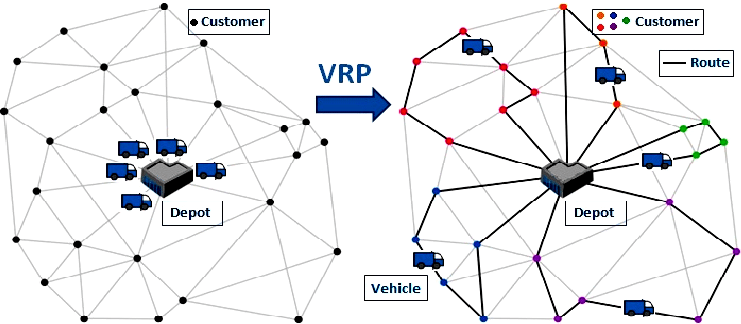
\includegraphics[width=.9\linewidth]{Classical-Vehicle-Routing-Problem.png}
    \end{center}
    {\footnotesize Gupta, Ashima \& Saini, Sanjay. (2017). An Enhanced Ant Colony Optimization Algorithm for Vehicle Routing Problem with Time Windows. 267-274. 10.1109/ICoAC.2017.8441175.}
\end{frame}

\begin{frame}{Formal definition}
    Let $G=(V,E)$ be a strongly connected, weighted, directed graph where
    \begin{itemize}
        {\parskip=0pt
        \item vertices represent intersecting roads and/or customers,
        \item all vertices possess latitude/longitude information $(x,y)$,
        \item all trucks start and end at a central warehouse described by a node $w\in V$,
        \item $C\subseteq V\setminus\{w\}$ is the set of customers (destinations) the trucks must visit,
        \item edges represent the existence of a road connecting two vertices where edge weights describe the distance between the two nodes.}
    \end{itemize}
    Let $T$ be a finite set of trucks each with fixed capacity $k$ where the total number of customers a single truck visits cannot exceed $k$. Additionally, ensure $|T|k\geq|C|$ so that all customers are fullfilled in a single round.

    We define function $\text{PARS}(G,w,C,T,k)$ which outputs a mapping $T\to\{(w,\dots,w)\subseteq V,\dots\}$ which describes the route of each truck starting at $w$ and ending at $w$. The goal of this function is to minimize the total distance traveled, the sum of edge weights, across all trucks.
\end{frame}

\section{Establishing a baseline}

\begin{frame}{Decomposing a VRP into multiple TSPs}
    A single vehicle routing problem can be thought of as a multi-agent traveling salesman problem. Solving this would be a lot easier if we could decompose a VRP into multiple TSPs we could solve individually, and moreover, in parallel.
    \begin{columns}[T,totalwidth=\textwidth]
        \begin{column}{.35\textwidth}
            \parskip=\defaultparskip
            We can achieve this by finding a way to partition the set of customers $C$ while also adhering to the truck capacity constraint $k$. Doing this reduces the complexity of our problem greatly.
        \end{column}
        \begin{column}{.65\textwidth}
            \centering
            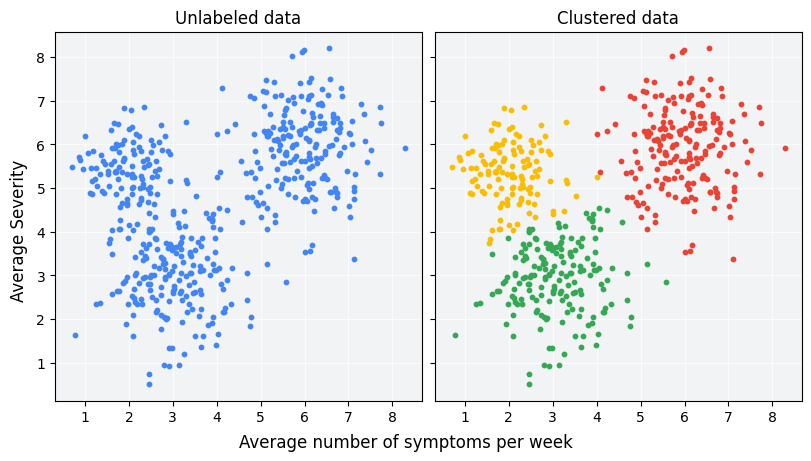
\includegraphics[width=.95\textwidth]{clustering_example.png}
        \end{column}
    \end{columns}
\end{frame}

\begin{frame}{Sweep algorithm}
    \begin{columns}
        \begin{column}{.6\linewidth}
            \parskip=\defaultparskip
            One such method to partition customers is sweeping. Conceptually, we draw a ray out from the central warehouse in some direction and ``sweep'' that ray around a full 360\textsuperscript{\circ}.

            As our ray sweeps around, we will pass over customers. When we hit a customer we allocate that customer to a truck, say truck 1. Once that truck is filled, we move onto allocating customers to truck 2, truck 3, and so on.

            In practice, we do this by calculating 2-argument arctangent of each customer, $\theta=\text{atan2}(\text{lat},\text{lon})$, sort all customers by this result, then allocate customers as mentioned above.
        \end{column}
        \begin{column}{.4\linewidth}
            \centering
            \animategraphics[width=\linewidth]{10}{sweep_algorithm_demo_frames/frame}{1}{96}

            {\footnotesize Sweep algorithm partitioning 32 customers among 4 trucks.}
        \end{column}
    \end{columns}
\end{frame}

\begin{frame}[plain]
    \begin{columns}
        \begin{column}{.4\linewidth}
            \parskip=\defaultparskip
            Here we see PARS executed on a $\qty{10}{\km}\times\qty{10}{\km}$ map of Albany, NY featuring 36 customers, 6 trucks, each with a capacity of 6.

            Each TSP is solved using nearest neighbor heuristic for customer selection and A* search (using Euclidean distance as heuristic) for routing.
        \end{column}
        \begin{column}{.6\linewidth}
            \centering
            \vfill
            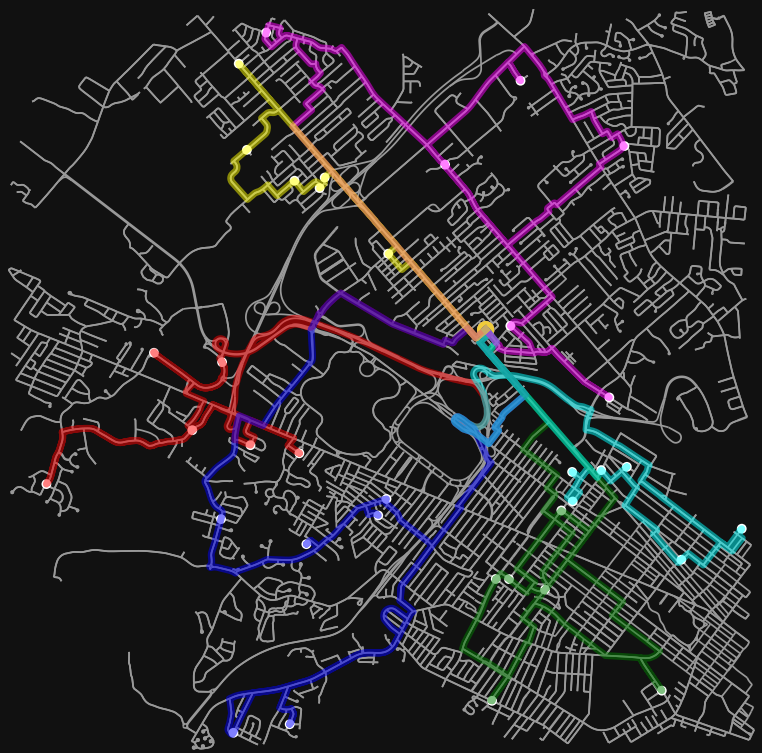
\includegraphics[width=.95\linewidth]{sweep_algorithm_example.png}
            \vfill
        \end{column}
    \end{columns}
\end{frame}

\begin{frame}{A note on evaluations}
    All evaluations in this presentation were performed on a $\qty{20}{\km}\times\qty{20}{\km}$ map of Albany, NY centered at University at Albany, SUNY. This does not imply the warehouse is located at the university, just that the map is centered there.

    Each CVRP instance is generated by first randomly picking a central warehouse location $w\in V$ and then randomly sampling customer locations of the remaining vertices from the map, $C\subseteq V\setminus\{w\}$.

    Additionally, each instance features $|T|=10$ trucks, each with a capacity of $k=10$, and the number of customers $|C|\in[1,100]$ is varied randomly over 250 iterations.

    PARS is then executed on each instance and the total distance traveled across all trucks is recorded for each instance.
\end{frame}

\begin{frame}[plain]
    \begin{center}
        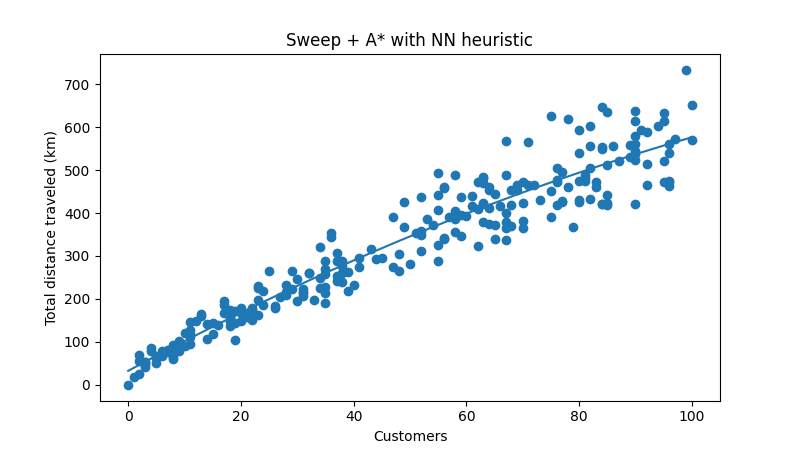
\includegraphics[width=\linewidth]{sweep_astar_nn.png}
    \end{center}
\end{frame}

\section{Improving the baseline}

\begin{frame}{Simulated annealing}
    \textbf{Simulated annealing} --- A randomized algorithm for approximating the global optimum of some function. It emulates the cooling of hot metal whereby early on the algorithm accepts longer routes to ``see where they might go''. Though, as we cool, we become more conservative.

    This technique is ideal for solving individual TSPs.

    \begin{center}
        \animategraphics[width=.65\linewidth]{24}{Hill_Climbing_with_Simulated_Annealing/frame}{1}{275}

        {\footnotesize Simulated annealing being used to search for a global maximum}
    \end{center}
\end{frame}

\begin{frame}{Obtaining a new state}
    Simulated annealing revolves around trying to optimize some state $s$. In our case the state is simply the route a single truck takes. For example,
    \[
        s=(w,c_1,c_2,c_3,w)
    \]
    where $w$ is the central warehouse and $c_i\in C$ denotes customers.

    Optimization is performed by obtaining a new state $s_\text{new}$ which is generated by slightly modifying the existing state, then comparing it against the existing best state.

    In our case, we generate our new state by randomly modifying the order in which a truck will visit each customer. We do this simply by picking two customers at random and swapping their order in $s$.

    For example, here's a new state where the truck now visits the second customer first then the first customer second.
    \[
        s_\text{new}=(w,c_2,c_1,c_3,w)
    \]
\end{frame}

\begin{frame}{Evaluation of a state and temperature}
    The \textbf{energy of a state}, denoted $E(s)\in\mathbb{R}$, is how we quantify the quality of a solution. This is the value we want to either minimize or maximize. In our case, we define $E(s)$ to be the total distance a truck will have to travel.

    To ensure we don't get stuck in local optimums, we introduce the concept of \textbf{temperature}. This value starts high and decays over time, by \textbf{decay rate} $u$. This temperature value ensures that we are more likely to accept worse solutions early on in the algorithm, but as we cool down, we become more conservative and less likely to accept worse solutions.

    In our case, we use an initial temperature of $T=10,000$ with a decay rate of $u=0.995$.
\end{frame}

\begin{frame}{Probability acceptance function}
    To bring this all together we introduce the \textbf{probability acceptance function}, denoted $P(e,e_{new},T)\in[0,1]$. This is the probability of making a transition from the current state $s$ to a new candidate state $s_\text{new}$. In our case we define $P$ as follows
    \[
        P(e,e_\text{new},T)=\begin{cases}
            1 & \text{if }e_\text{new}<e \\
            \displaystyle\exp\left(\frac{-(e_\text{new}-e)}{T}\right) & \text{otherwise}
        \end{cases}
    \]
    This probability acceptance function is key as this is what compares the quality of a new solution with the algorithm's current temperature. Here we see that if we find a more optimal solution (first condition), we always use that instead, however, if we find a less optimal solution (second condition), we may switch to it depending on how much better it is, $e_\text{new}-e$, and what the current temperature $T$ is.
\end{frame}

\begin{frame}[plain]
    \begin{columns}
        \begin{column}{.4\linewidth}
            Here we see simulated annealing in action. It is being used to solve a 10 customer TSP over Albany, NY.
        \end{column}
        \begin{column}{.6\linewidth}
            \centering
            \animategraphics[width=\linewidth]{3}{annealing_demo/route}{1}{16}
        \end{column}
    \end{columns}
\end{frame}

\begin{frame}[plain]
    \begin{center}
        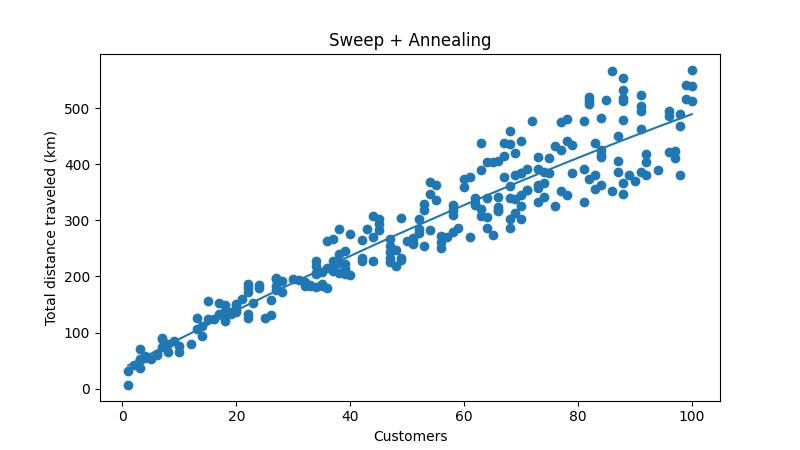
\includegraphics[width=\linewidth]{sweep_annealing.png}
    \end{center}
\end{frame}

\begin{frame}[plain]
    \centering
    
\includegraphics[width=\linewidth]{comparison.png}
\end{frame}

\begin{frame}{Conclusion}
    \begin{enumerate}
        \item We established a baseline by decomposing our VRP into multiple TSPs using the sweep algorithm, then solving each TSP using nearest neighbor heuristic for customer selection and A* search for routing.
        \item We improved our baseline by using simulated annealing to solve each TSP instead of nearest neighbor heuristic.
        \item Simulated annealing does offer an improvement over nearest neighbor heuristic for solving TSPs. It managed to achieve a 22\% improvement over our baseline, at best.
        \item Moving forward, we want to collect more statistics across wider data sets, investigate other optimization techniques as well as analyzing where certain techniques perform better than others.
    \end{enumerate}
\end{frame}

\begin{frame}[plain]
    \centering\LARGE\textbf{Thank you!}
\end{frame}

\end{document}
